%!TEX root = ../../main.tex

\chapter{Fabrication of \Nds}	\label{ch::fabrication_nanodiamonds}
\chaptermark{Fabrication of \Nds}

	% \epigraph{``Diamond forms under high temperature and pressure conditions that exist only about 100 miles beneath the earth's surface.''}{\textup{Gemological Institute of America Inc.}}

	Due to its extraordinary properties, diamond has transcended its sole purpose as a rare gem and developed into an important tool enabling various applications in industry and research. This change has been driven largely by the development of methods allowing to cheaply produce synthetic diamond. While synthetic diamonds are typically small and without the splendor generally associated with diamond, they can be produced on-demand and are thus arguably more useful than rare gemstones.
	In this chapter we introduce the two most common methods for the fabrication of diamonds in a laboratory setting: The \hpht and the \cvd method.
	The aptly named \hpht (\HPHT) process mimics the conditions under which diamond is formed in nature and is widely used to synthetically produce diamonds for industrial applications such as utilization of diamond as a abrasive.
	While \HPHT diamonds are utilized in this work, most reported measurements are based on diamond produced with the \CVD method in which diamonds are grown using a hydrocarbon gas mixture. Both processes have in common that defects and impurities are a naturally occurring.
	For a more extensive list of diamond production processes refer to \cite{davis1993diamond}.
	In the context of this thesis nano-sized diamonds are required. They can be obtained by milling larger sized \HPHT or \CVD diamonds down to the desired grain size in a vibrational mill.
	The obtained \nds are small enough that individual specimen have a chance of hosting a singleton \siv. These can be identified and used for further exploration.

\section[HPHT]{High-Pressure High-Temperature Diamond}\label{sec::hpht}

	The \HPHT method was the first process to successfully synthesize diamond in 1879.
	Today, it is still widely used due to its relatively cheap production costs for small diamonds.
	\\
	In the \HPHT process, diamond is synthesized from graphite under temperatures of up to \SI{1.5d3}{\celsius} pressures between \SI{5d4}{bar} and \SI{d6}{bar} \cite{davis1993diamond}. Under these extreme conditions, carbon transitions from its graphite to its diamond phase because the latter becomes energetically favorable \cite{liander1955artificial, bundy1955man, bovenkerk1993errors, bovenkerk1959preparation}.
	The machine used for this kind of synthesis is a press.
	For some forms of this method, a metallic catalyst solvent is added lowering the required pressures and temperatures by causing graphite to dissolve earlier. At the same the catalyst promotes the crystallization process.
	Several press designs exist, all of which relying on creating and maintaining high pressures and a high temperatures.
	While it is possible to grow big ($> \SI{10}{\carat}$) high-quality diamonds with the \HPHT process, its cost quickly increases and thus becomes unfavorable.
	\\
	In this thesis, \HPHT \nds diamonds produced by Davydov et al. \cite{Davydov2014} are spectroscopically investigated.

\section[CVD]{Chemical Vapor Deposition Diamond}\label{sec::cvd}

	In contrast to the \HPHT method, diamond is crystallized from carbon available in the gas phase in the \CVD method.
	The process still requires respectable temperatures in the range of \SIrange{700}{1300}{\celsius} but makes due with the low pressures of less than \SI{1}{\bar} available in a vacuum growth chamber \cite{schwander2011review}.
	\\
	The chamber contains a vapor consisting of a mixture of atomic hydrogen and methane. The gas can be forced into the plasma phase using strong microwaves or hot filaments \cite{balmer2009chemical, ferro2002synthesis, koizumi2008physics}. While the hot filament is easy to implement, it has the disadvantage that atoms which are etched from the filament during the growth process are likely to contaminate the diamond. To minimize the introduction of defects other than \sivs in the diamond, growing diamonds in a microwave plasma is preferred. In it methane molecules dissociate and relase carbon. In the presence of a substrate such as \ir containing suitable seeds, carbon can crystallize forming diamond. \Fref{fig::cvd_sketch} illustrates the setup. In a plasma containing atomic hydrogen, the formation of diamond is favored over the formation of graphite. This is due to the fact that the atomic hydrogen preferentially etches sp$^2$ bonded carbon, i.e.\ graphite.

	\begin{figure}[htp]
		\centering
		\testbox{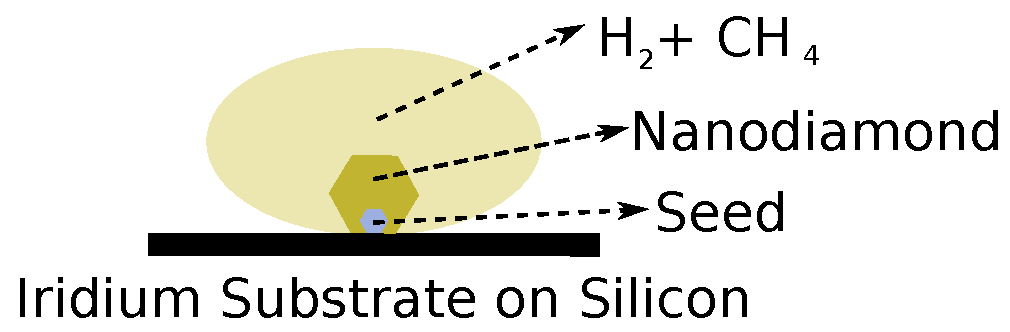
\includegraphics[trim = 0 0 0 0,  clip= true, width = 0.3\textwidth]{./pics/cvd_sketch.pdf}}
		\caption[\CVD production method]{Sketch of the \CVD method. A hydrogen-carbon plasma acts as a donor for carbon atoms which may crystallize to form diamond on-top of a suitable \ir substrate. An initial diamond seed facilitates the process.}
		\label{fig::cvd_sketch}
	\end{figure}

	Typically, single crystal diamond substrates are required to grow single crystal diamond. \HPHT substrates are suitable to start a crystallization process. This approach is referred to as homoepitaxial growth. An alternative approach is to utilize non-diamond substrates such as \ir or platinum to trigger heteroepitaxial growth \cite{tachibana2001growth, lin1994local}.
	This method is utilized for all the \CVD \nds grown and investigated in this thesis.
	It relies on small diamond crystals deposited in the substrate acting as seeds for the diamond crystallization process\footnote{\CVD \nd growth performed by \gsell}. Seed diamond crystals are commercially available, and are usually particles produced by a so-called detonation process.
	In a detonation process, the high pressure produced by shock-waves of a detonation is used to create very small diamond particles of a size down to a few nanometers.
	
	Growth on a substrate is favored, if the lattice constant of the substrate and the diamond to be grown are similar.
	The lattice constant of \ir is \SI{0.384}{nm} \cite{Arblaster2010,Gsell2007} and thus close to the lattice constant of diamond with \SI{0.356}{nm} \cite{davis1993diamond}.
	Therefore, the diamond was grown on a stratified substrate topped with an \ir layer of \SIrange{60}{150}{nm} thickness\footnote{Production of the stratified substrate performed by \gsell}.
	The \ir layers themselves were grown onto an yttria-stabilized zirconia (YSZ) buffer layer, which in turn was grown on a silicon wafer \cite{Gsell2004a}.
	If the lattice constant of the substrate and the diamond are not matched, stress in the diamond lattice is induced.
	Therefore, the \ir substrate not only facilitates diamond growth, but also reduces unfavorable stress in the \nds. The detrimental effects of stress on the diamond lattice and its implications with respect to hosted \sivs are briefly discussed in \Fref{ch::distribution}.
?